\documentclass{article}
\usepackage{listings}
\usepackage{hyperref}
\usepackage{graphicx}
\usepackage{float}
\begin{document}
\title{EOPSY Lab 3 Report}
\author{Krzysztof Rudnicki, 307585}
\date{\today}
\maketitle
\section{Introduction}
ALL TEXT SURROUNDED BY [] LIKE \cite{lab3 Manual} SHOULD BE CLICKABLE AND LEAD
EITHER TO WEBPAGE OR PLACE IN THIS DOCUMENT \\
The goal of the laboratory was to create three scenarios using config file and
then investigate how those scenarios played out. \\
Scenario 1: 2 Processes \\
Scenario 2: 5 Processes \\
Scenario 3: 10 Processes \\
We had to get to know how the schedulers work, how they switch. \cite{lab3
Manual} 
\paragraph{First come first serve}
We used First come first serve algorithm $\rightarrow$ This algorithm simply executes the process which
arrived first. The process that requests CPU as a first process gets the CPU
first. It is easy to implement and understand. We just use Queue data structure
and we pick processes from the head of the queue and new procesess are added at
the tail of the queue. \cite{First come first serve}
\begin{figure}[H]
	\caption{First come first serve example graphic from
		\href{https://www.geeksforgeeks.org/program-for-fcfs-cpu-scheduling-set-1/}{[Geeks for
	Geeks]}}
	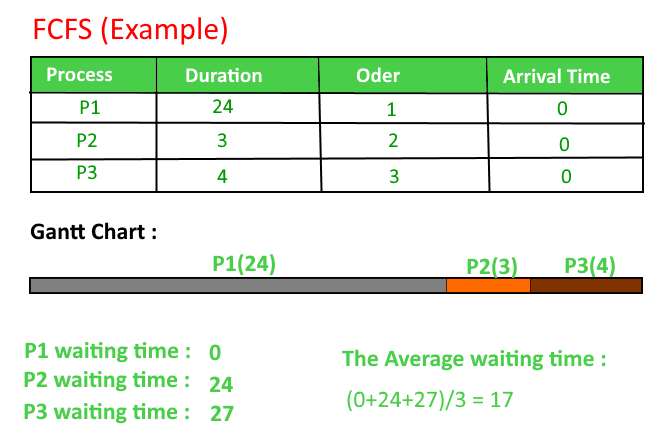
\includegraphics[width=\textwidth]{FCFS}
\end{figure}
\paragraph{Other algorithms} \cite{Other scheduling algorithms}
\begin{enumerate}
	\item Shortest-Job-Next - Executes first processes that will take least
		time to finish
	\item Priority Scheduling - Each process gets assigned a prority and we
		execute them from the process with highest priority to the
		process with lowest prority
	\item Round Robin Scheduling - We give each process a constant time to
		execute, after this time expires regardless whether process
		finished or not we go to another process untill all of them are
		finished
\end{enumerate}
\section{Explanation of types of values in summary results and summary
process} 
\subsection{Summary Results} 
\begin{itemize}
	\item Scheduling Type - Type of scheduling algorithm used
	\item Scheduling Name - Name of the scheduling algorithm
	\item Simulation Run Time - How long simulation run
	\item Mean - Average runtime for the processes
	\item Standard Deviation - Deviation from mean
	\item Process \#    - Process number
	\item CPU Time      - Total runtime for the process
	\item IO Blocking   - How long process runs before it is blocked for
		input or output
	\item CPU Completed - How long runtime completed for the process
	\item CPU Blocked   - How often the process was blocked
\end{itemize}
\cite{lab3 Manual}
\subsection{Summary Processes} 
\begin{itemize}
	\item process-number - Process number assigned by simulator
	\item process-status - Registered - process can be used by scheduling
		algorithm, I/O blocked - process blocked for input or output,
		Completed - process met or exceeded execution time
	\item cpu-time - Total amount of runtime allowed for this process
	\item block-time - amount of time before blocking process
	\item accumulated-time - how long the process has already executed
		(appears twice)
\end{itemize}
\cite{lab3 Manual}

\section{Scheduling conf settings}
\begin{lstlisting}
// # of Process	
numprocess 2 or 5 or 10

// mean deivation
meandev 2000

// standard deviation
standdev 0

// process    # I/O blocking
process 500
process 500
(more if we set numprocess to 5 or 10)

// duration of the simulation in milliseconds
runtime 10000

\end{lstlisting}

\section{Two processes}
\subsection{Summary Results file}


\begin{lstlisting}
Scheduling Type: Batch (Nonpreemptive)
Scheduling Name: First-Come First-Served
Simulation Run Time: 4000
Mean: 2000
Standard Deviation: 0
\end{lstlisting}

\begin{center}
\begin{tabular}{| c | c | c | c | c |}
\hline
Process\# &	CPU Time &	IO Blocking & CPU Completed & CPU Blocked \\
\hline
0&		2000 (ms)&	500 (ms)&	2000 (ms)&	3 times \\
\hline
1&		2000 (ms)&	500 (ms)&	2000 (ms)&	3 times \\
\hline
\end{tabular}
\end{center}

\subsection{Summary Processes file}
\begin{lstlisting}
Process: 0 registered... (2000 500 0 0)
Process: 0 I/O blocked... (2000 500 500 500)
Process: 1 registered... (2000 500 0 0)
Process: 1 I/O blocked... (2000 500 500 500)
Process: 0 registered... (2000 500 500 500)
Process: 0 I/O blocked... (2000 500 1000 1000)
Process: 1 registered... (2000 500 500 500)
Process: 1 I/O blocked... (2000 500 1000 1000)
Process: 0 registered... (2000 500 1000 1000)
Process: 0 I/O blocked... (2000 500 1500 1500)
Process: 1 registered... (2000 500 1000 1000)
Process: 1 I/O blocked... (2000 500 1500 1500)
Process: 0 registered... (2000 500 1500 1500)
Process: 0 completed... (2000 500 2000 2000)
Process: 1 registered... (2000 500 1500 1500)
Process: 1 completed... (2000 500 2000 2000)
\end{lstlisting}
\subsection{Comments}
Scheduling type was Batch since I did not change it in SchedulingAlgorithm.java
file \\
Scheduling Name was First-Come First-Served since this is what what we use as
described in README for this laboratory \\
Simulation Run time is 4000 ms and NOT 10000 ms since the simulation finished
before it exceeded this max time \\
Mean is 2000 since this is a value I set in conf value according to laboratory
task description, same with standard deviation equal to 0 and CPU Time equal to
2000 ms \\
IO Blocking is equal to 500 ms, this is a value which we specified in
configuration file and since we did not exceeded the runtime parameter it stayed
equal to 500 ms \\
CPU completed is equal to 2000 since this is deviation we set in configuration
settings and the runtime was not exceeded \\
All processes blocked 3 times, analysing summary processes we can see that they
blocked at 500 ms, 1000 ms and 1500 ms and at 2000 seconds they completed 
 
\section{Five processes}
\newpage
\subsection{Summary Results file}
\begin{lstlisting}
Scheduling Type: Batch (Nonpreemptive)
Scheduling Name: First-Come First-Served
Simulation Run Time: 10000
Mean: 2000
Standard Deviation: 0
\end{lstlisting}
\begin{center}                        
\begin{tabular}{| c | c | c | c | c |}                                      
\hline                                                                      
Process\# &     CPU Time &      IO Blocking & CPU Completed & CPU Blocked \\
\hline
0&		2000 (ms)&	500 (ms)&	2000 (ms)&	3 times \\
\hline
1&		2000 (ms)&	500 (ms)&	2000 (ms)&	3 times \\
\hline
2&		2000 (ms)&	500 (ms)&	2000 (ms)&	3 times \\
\hline
3&		2000 (ms)&	500 (ms)&	2000 (ms)&	3 times \\
\hline
4&		2000 (ms)&	500 (ms)&	2000 (ms)&	3 times \\
\hline
\end{tabular}
\end{center}
           
\subsection{Summary Processes file}
\begin{lstlisting}
Process: 0 registered... (2000 500 0 0)
Process: 0 I/O blocked... (2000 500 500 500)
Process: 1 registered... (2000 500 0 0)
Process: 1 I/O blocked... (2000 500 500 500)
Process: 0 registered... (2000 500 500 500)
Process: 0 I/O blocked... (2000 500 1000 1000)
Process: 1 registered... (2000 500 500 500)
Process: 1 I/O blocked... (2000 500 1000 1000)
Process: 0 registered... (2000 500 1000 1000)
Process: 0 I/O blocked... (2000 500 1500 1500)
Process: 1 registered... (2000 500 1000 1000)
Process: 1 I/O blocked... (2000 500 1500 1500)
Process: 0 registered... (2000 500 1500 1500)
Process: 0 completed... (2000 500 2000 2000)
Process: 1 registered... (2000 500 1500 1500)
Process: 1 completed... (2000 500 2000 2000)
Process: 2 registered... (2000 500 0 0)
Process: 2 I/O blocked... (2000 500 500 500)
Process: 3 registered... (2000 500 0 0)
Process: 3 I/O blocked... (2000 500 500 500)
Process: 2 registered... (2000 500 500 500)
Process: 2 I/O blocked... (2000 500 1000 1000)
Process: 3 registered... (2000 500 500 500)
Process: 3 I/O blocked... (2000 500 1000 1000)
Process: 2 registered... (2000 500 1000 1000)
Process: 2 I/O blocked... (2000 500 1500 1500)
Process: 3 registered... (2000 500 1000 1000)
Process: 3 I/O blocked... (2000 500 1500 1500)
Process: 2 registered... (2000 500 1500 1500)
Process: 2 completed... (2000 500 2000 2000)
Process: 3 registered... (2000 500 1500 1500)
Process: 3 completed... (2000 500 2000 2000)
Process: 4 registered... (2000 500 0 0)
Process: 4 I/O blocked... (2000 500 500 500)
Process: 4 registered... (2000 500 500 500)
Process: 4 I/O blocked... (2000 500 1000 1000)
Process: 4 registered... (2000 500 1000 1000)
Process: 4 I/O blocked... (2000 500 1500 1500)
Process: 4 registered... (2000 500 1500 1500)
\end{lstlisting}    
\subsection{Comments}
Scheduling type was Batch since I did not change it in SchedulingAlgorithm.java
file \\
Scheduling Name was First-Come First-Served since this is what what we use as
described in README for this laboratory \\
Simulation run time is 10000 ms since it run untill the limit I set in conf file
according to task description \\
CPU blocking is set everywhere to 500 ms as in conf file \\
Mean is 2000 since this is a value I set in conf value according to laboratory
task description, same with standard deviation equal to 0 and CPU Time equal to
2000 ms \\
CPU completed is equal to expected 2000 ms, this makes sense since we had run
time equal to 10000 ms and 5 procesess so each of them could take exactly the
amonunt of time we set them to take.


\section{Ten processes}
\subsection{Summary Results file}                                              
\begin{lstlisting}
Scheduling Type: Batch (Nonpreemptive)
Scheduling Name: First-Come First-Served
Simulation Run Time: 10000
Mean: 2000
Standard Deviation: 0
\end{lstlisting}
\begin{center}                                                                 
\begin{tabular}{| c | c | c | c | c |}                                         
\hline                                                                         
Process\# &     CPU Time &      IO Blocking & CPU Completed & CPU Blocked \\
\hline
0		&2000 (ms)	&500 (ms)&	2000 (ms)&	3 times \\
\hline
1		&2000 (ms)	&500 (ms)&	2000 (ms)&	3 times \\
\hline
2		&2000 (ms)	&500 (ms)&	2000 (ms)&	3 times \\
\hline
3		&2000 (ms)	&500 (ms)&	2000 (ms)&	3 times \\
\hline
4		&2000 (ms)	&500 (ms)&	1000 (ms)&	2 times \\ 
\hline
5		&2000 (ms)	&500 (ms)&	1000 (ms)&	1 times \\
\hline
6		&2000 (ms)	&500 (ms)&	0 (ms)&		0 times \\
\hline
7		&2000 (ms)	&500 (ms)&	0 (ms)&		0 times \\
\hline
8		&2000 (ms)	&500 (ms)&	0 (ms)&		0 times \\
\hline
9		&2000 (ms)	&500 (ms)&	0 (ms)&		0 times \\
\hline
\end{tabular}
\end{center}
\subsection{Summary Processes file}
\begin{lstlisting}         
Process: 0 registered... (2000 500 0 0)
Process: 0 I/O blocked... (2000 500 500 500)
Process: 1 registered... (2000 500 0 0)
Process: 1 I/O blocked... (2000 500 500 500)
Process: 0 registered... (2000 500 500 500)
Process: 0 I/O blocked... (2000 500 1000 1000)
Process: 1 registered... (2000 500 500 500)
Process: 1 I/O blocked... (2000 500 1000 1000)
Process: 0 registered... (2000 500 1000 1000)
Process: 0 I/O blocked... (2000 500 1500 1500)
Process: 1 registered... (2000 500 1000 1000)
Process: 1 I/O blocked... (2000 500 1500 1500)
Process: 0 registered... (2000 500 1500 1500)
Process: 0 completed... (2000 500 2000 2000)
Process: 1 registered... (2000 500 1500 1500)
Process: 1 completed... (2000 500 2000 2000)
Process: 2 registered... (2000 500 0 0)
Process: 2 I/O blocked... (2000 500 500 500)
Process: 3 registered... (2000 500 0 0)
Process: 3 I/O blocked... (2000 500 500 500)
Process: 2 registered... (2000 500 500 500)
Process: 2 I/O blocked... (2000 500 1000 1000)
Process: 3 registered... (2000 500 500 500)
Process: 3 I/O blocked... (2000 500 1000 1000)
Process: 2 registered... (2000 500 1000 1000)
Process: 2 I/O blocked... (2000 500 1500 1500)
Process: 3 registered... (2000 500 1000 1000)
Process: 3 I/O blocked... (2000 500 1500 1500)
Process: 2 registered... (2000 500 1500 1500)
Process: 2 completed... (2000 500 2000 2000)
Process: 3 registered... (2000 500 1500 1500)
Process: 3 completed... (2000 500 2000 2000)
Process: 4 registered... (2000 500 0 0)
Process: 4 I/O blocked... (2000 500 500 500)
Process: 5 registered... (2000 500 0 0)
Process: 5 I/O blocked... (2000 500 500 500)
Process: 4 registered... (2000 500 500 500)
Process: 4 I/O blocked... (2000 500 1000 1000)
Process: 5 registered... (2000 500 500 500)
\end{lstlisting}     
\subsection{Comments}
Scheduling type was Batch since I did not change it in SchedulingAlgorithm.java
file \\
Scheduling Name was First-Come First-Served since this is what what we use as
described in README for this laboratory \\
Simulation run time is 10000 ms since it run untill the limit I set in conf file
according to task description \\
IO Blocking set to 500 ms as in config file \\
Mean is 2000 since this is a value I set in conf value according to laboratory
task description, same with standard deviation equal to 0 and CPU Time equal to
2000 ms \\
CPU completed this time is equal to 2000 up to 4th process and then is equal to
1000 ms for 5th and 6th and then it is equal to 0 ms, this means that the
simulation exceeded the runtime before it had a chance to run all processes

\section{Getting process to be blocked 4 times}
Up untill now process got blocked for maximum of 3 times. This makes sense since
since they get blocked every 500 ms and the runtime for single process is 2000
ms, so they get blocked first time at 500 ms, second time at 1000 ms and third
time at 1500 ms, at 2000 ms they finish execution so they do not get blocked. \\
If we change runtime of process to 2001 ms we should get as the result them
getting blocked 4 times! \\
I changed meandev in scheduling.conf to 2001 and observed results:
\subsection{Summary Results file}
\begin{lstlisting}
Scheduling Type: Batch (Nonpreemptive)
Scheduling Name: First-Come First-Served
Simulation Run Time: 6003
Mean: 2001
Standard Deviation: 0
\end{lstlisting}
\begin{center}
	\begin{tabular}{| c | c | c | c | c |}
		\hline
		Process \#&	CPU Time&	IO Blocking&	CPU Completed&
		CPU Blocked \\ \hline
		0	&	2001 (ms)&	500 (ms)&	2001 (ms)&
		4 times  \\ \hline
		1	&	2001 (ms)&	500 (ms)&	2001 (ms)&
		4 times \\ \hline
		2	&	2001 (ms)&	500 (ms)&	2001 (ms)&
		4 times \\ \hline
\end{tabular}
\end{center}
Sure enough we got all of the processes blocked 4 times!
\section{Finishing comments}
We runned all the processes, get to know scheduling, get to know first come
first served algorithm. \\
There are upsides and downsides of first come first served algorithm:
\\
Upsides:
\begin{itemize}
	\item It is easy to implement
	\item It is easy to understand
\end{itemize}
Downsides:
\begin{itemize}
	\item It is very inefficient (Last experiment with 10 processes barely
		acknowledged existence of the 5th one)
	\item High average wait time (Imagine 1000 processes and how long we
		would have to wait)
\end{itemize}
Using pretty much any other algorithm we could get better results \cite{First
come first serve}
\begin{figure}[H]
	\caption{\href{https://commons.wikimedia.org/wiki/File:Process_states.svg}{[Process
	states and how they switch from wikimedia]}}
	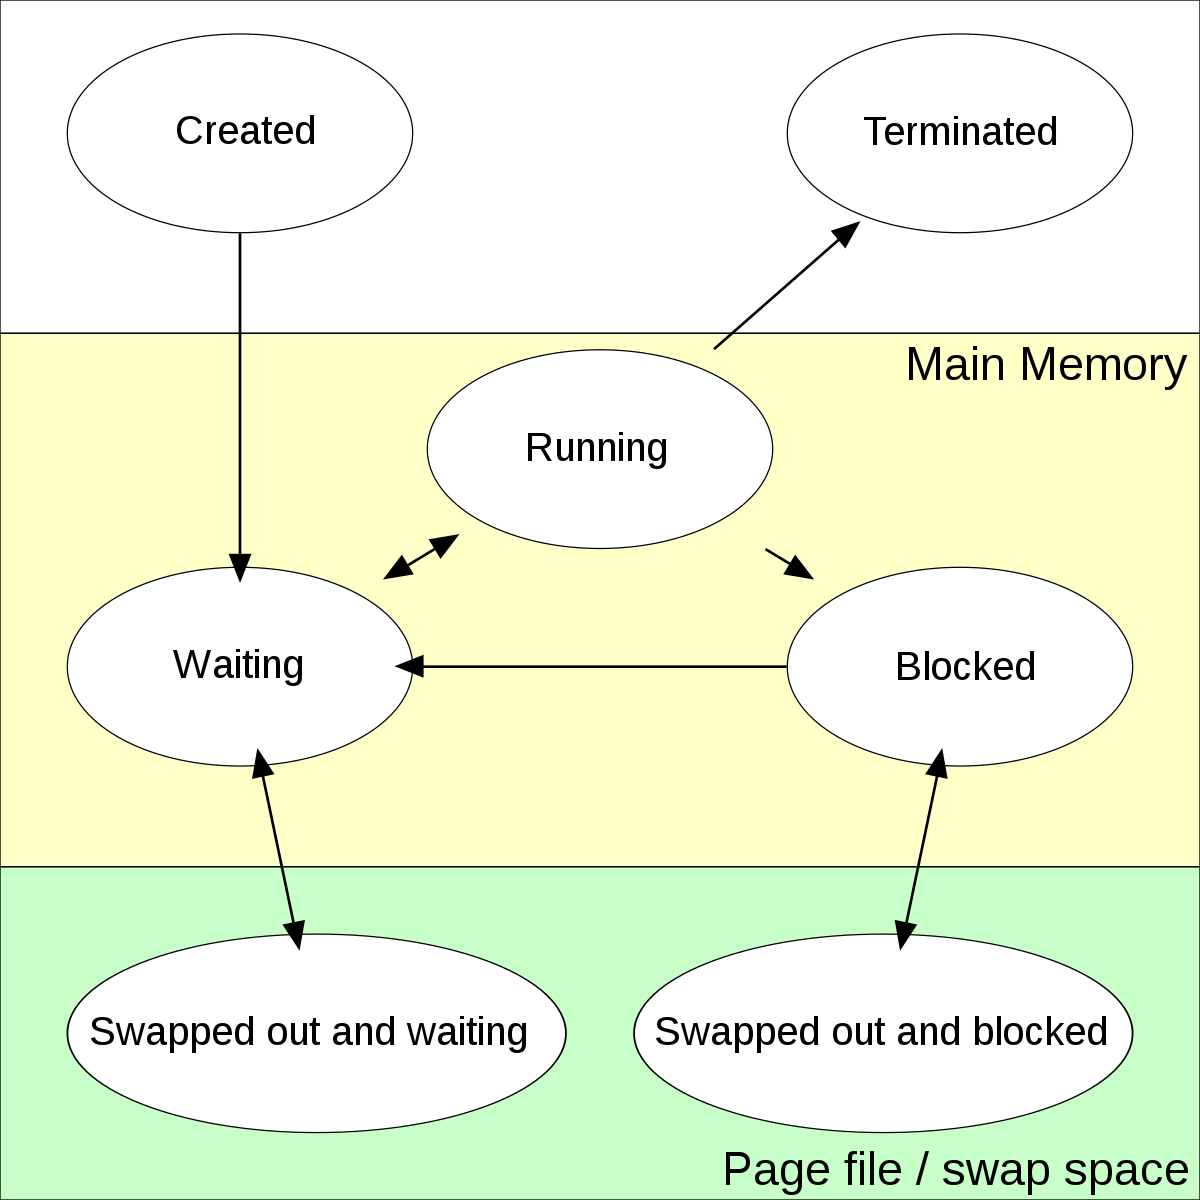
\includegraphics[width=\textwidth]{procestates}
\end{figure}

\begin{thebibliography}{9}
	\bibitem{lab3 Manual} Manual in the laboratory 3 files.
	\bibitem{First come first serve}
	\href{https://www.studytonight.com/operating-system/first-come-first-serve}{[https://www.studytonight.com/operating-system/first-come-first-serve]}
	\bibitem{Other scheduling algorithms}
	\href{https://www.tutorialspoint.com/operating_system/os_process_scheduling_algorithms.htm}{[Tutorials
point process scheduling algorithms]}
\end{thebibliography}
\end{document}
